\documentclass[letterpaper,12pt]{article}
\usepackage{tabularx} % extra features for tabular environment
\usepackage{amsmath}  % improve math presentation
\usepackage{float}
\usepackage{pdfpages}

\usepackage{graphicx} % takes care of graphic including machinery
\graphicspath{ {./figures/} }
\usepackage[margin=1in,letterpaper]{geometry} % decreases margins
\usepackage{cite} % takes care of citations
\usepackage[final]{hyperref} % adds hyper links inside the generated pdf file
\hypersetup{
	colorlinks=true,       % false: boxed links; true: colored links
	linkcolor=blue,        % color of internal links
	citecolor=blue,        % color of links to bibliography
	filecolor=magenta,     % color of file links
	urlcolor =blue         
}

%
\setcounter{tocdepth}{4} 
\setcounter{secnumdepth}{4}


\begin{document}

\title{Experiment 8 \protect\\First Order Circuits}
\author{Ahmet Akman 2442366 }
\date{\today}
\maketitle
\newpage
\tableofcontents
\newpage
%\begin{abstract}
%abstract
%\end{abstract}

\section{Introduction} 
In this experiment, as students, we are expected to experiment with first order circuits by completing the steps described in the eight experiment laboratory manual. The simple RC and RL circuit structures are expected to be learned throughout the first step. The output versus input characteristics ,and \(\tau\) value are obtained by connecting the signal generator to the oscilloscope and the circuit . Then, characteristics of variable \(\tau\) value is expected to be expressed and experimented. The results of the steps are recorded and plotted for further comments.
\section{Experimental Results}
In this section, the results of Experiment 8 are discussed. 
\subsection{Step 1}
In this step, circuit shown in the Figure 1  is constructed. 
\begin{figure}[H]
	\centering
   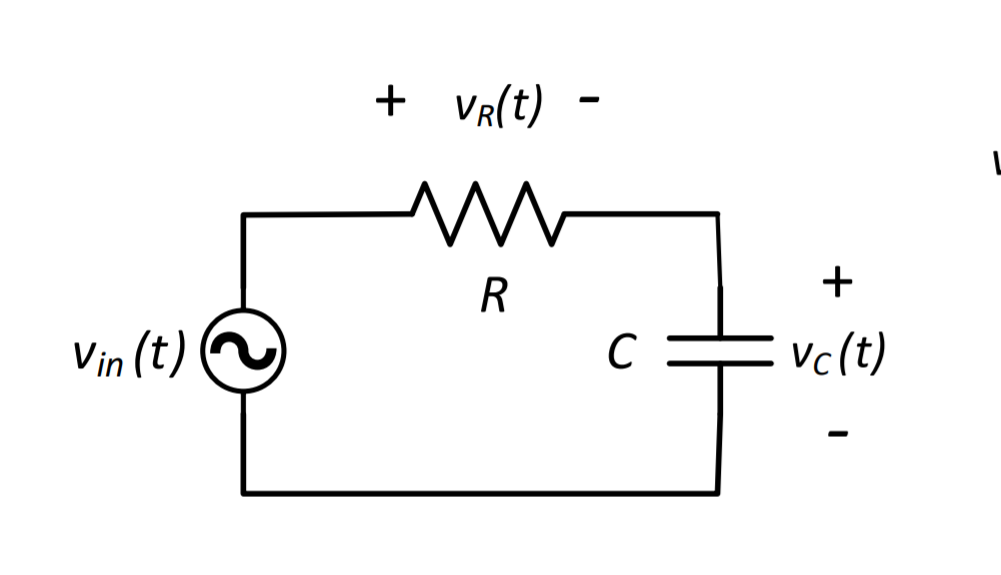
\includegraphics[width=0.8\textwidth]{1_sch.png}
   \caption{Circuit schematic for the step 1}
\end{figure} 
The square waveform generator is adjusted as given in Figure 2.
\begin{figure}[H]
	\centering
   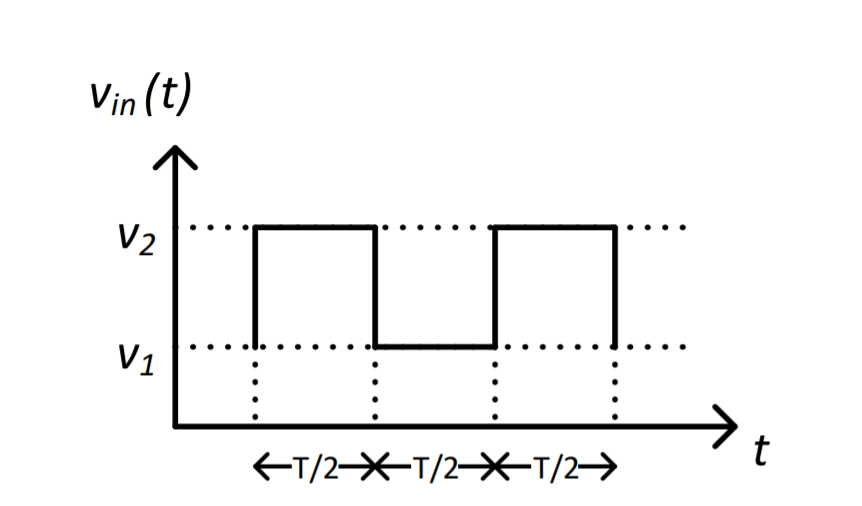
\includegraphics[width=0.8\textwidth]{1_signal.png}
   \caption{Waveform for the step 1}
\end{figure} 


\subsubsection{a)}
The set of data given in Table 1 is used for the measurements.

\begin{table}[H]
\begin{center}
\caption{RC circuit parameters}
\vspace{2mm}
	\begin{tabular}{||c | c | c | c||} 
	 \hline
	 \emph{f} (kHz) & R (k\(\Omega\)) & C (nF) & Theoretical Calculation \(\tau\) (\(\mu\) sec) \\ [0.5ex] 
	 \hline\hline
	 2 & 3.3 & 4.7 & 15.51 \\ 
	 \hline
	 2& 68 & 10  & 680  \\
	 \hline
\end{tabular}
\end{center}
\end{table}
The theoretical calculation of \(\tau\) is obtained from the general time constant equation of RC circuits;
\[\tau = R \times C\]
The result of the circuit with parameters of first row is given in Figure 3.

\begin{figure}[H]
	\centering
   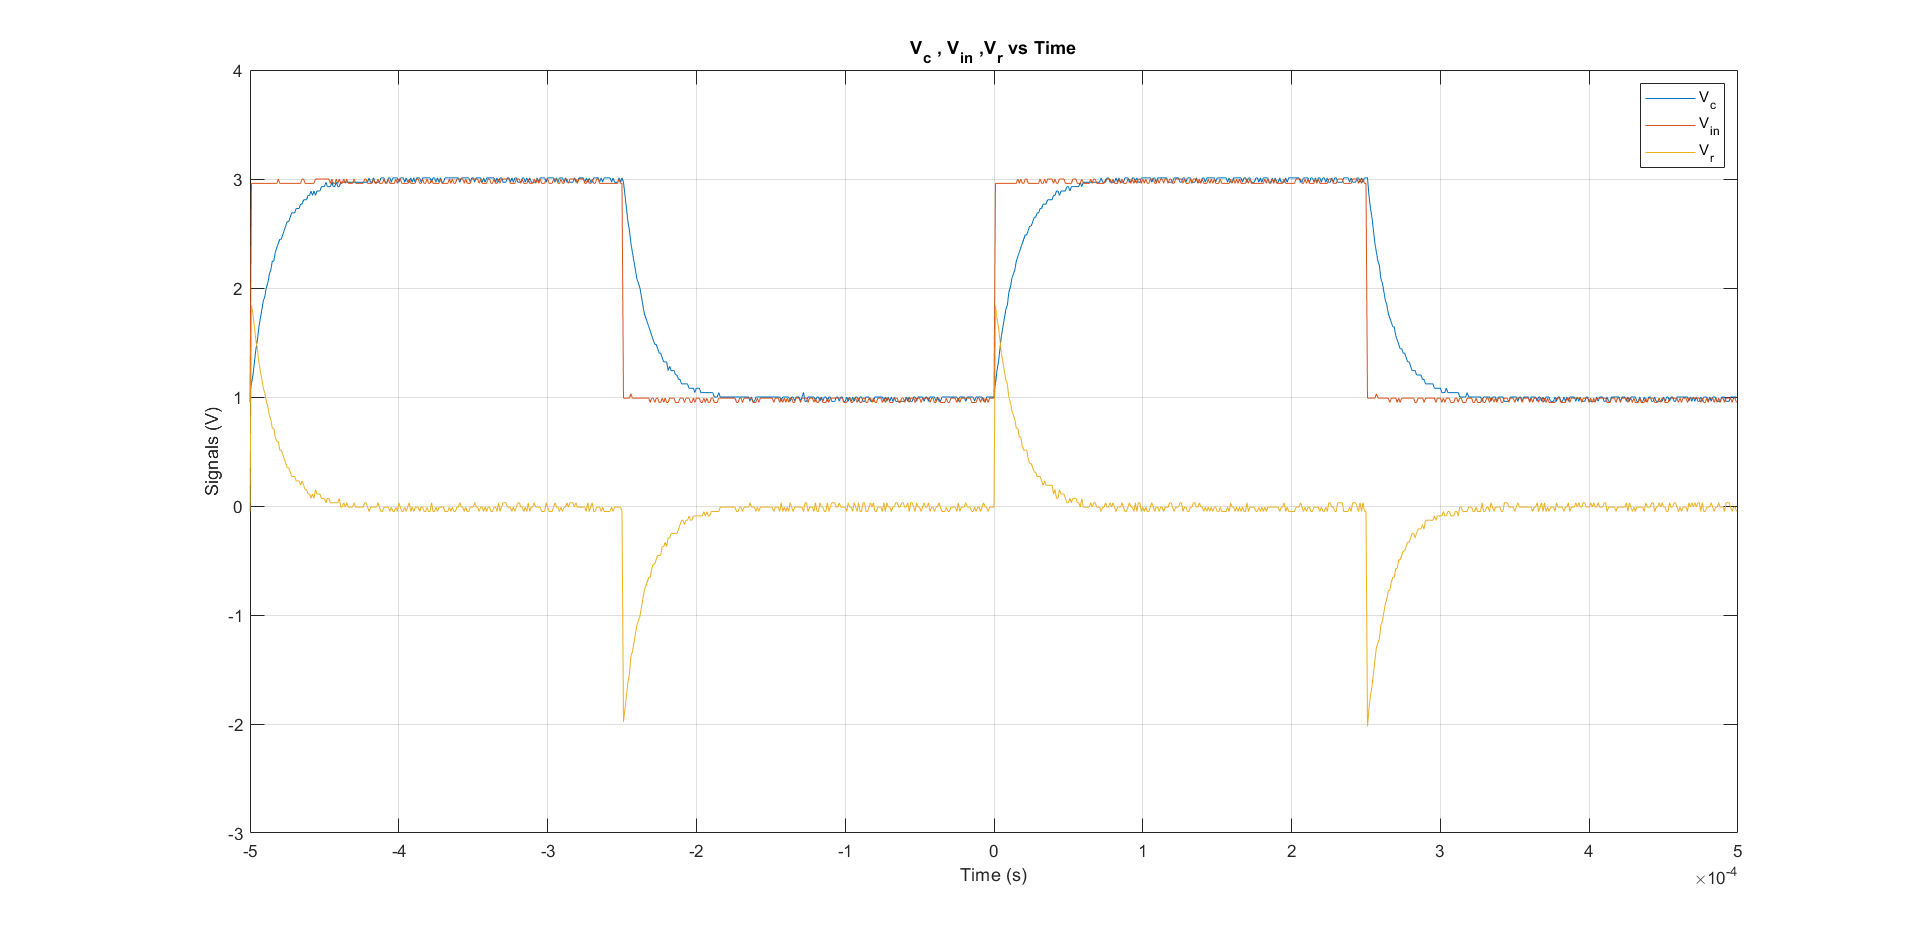
\includegraphics[width=0.8\textwidth]{1a.png}
   \caption{Waveform for the step 1}
\end{figure} 
To measure time constant experimentally following data is obtained from the plot.
\begin{figure}[H]
	\centering
   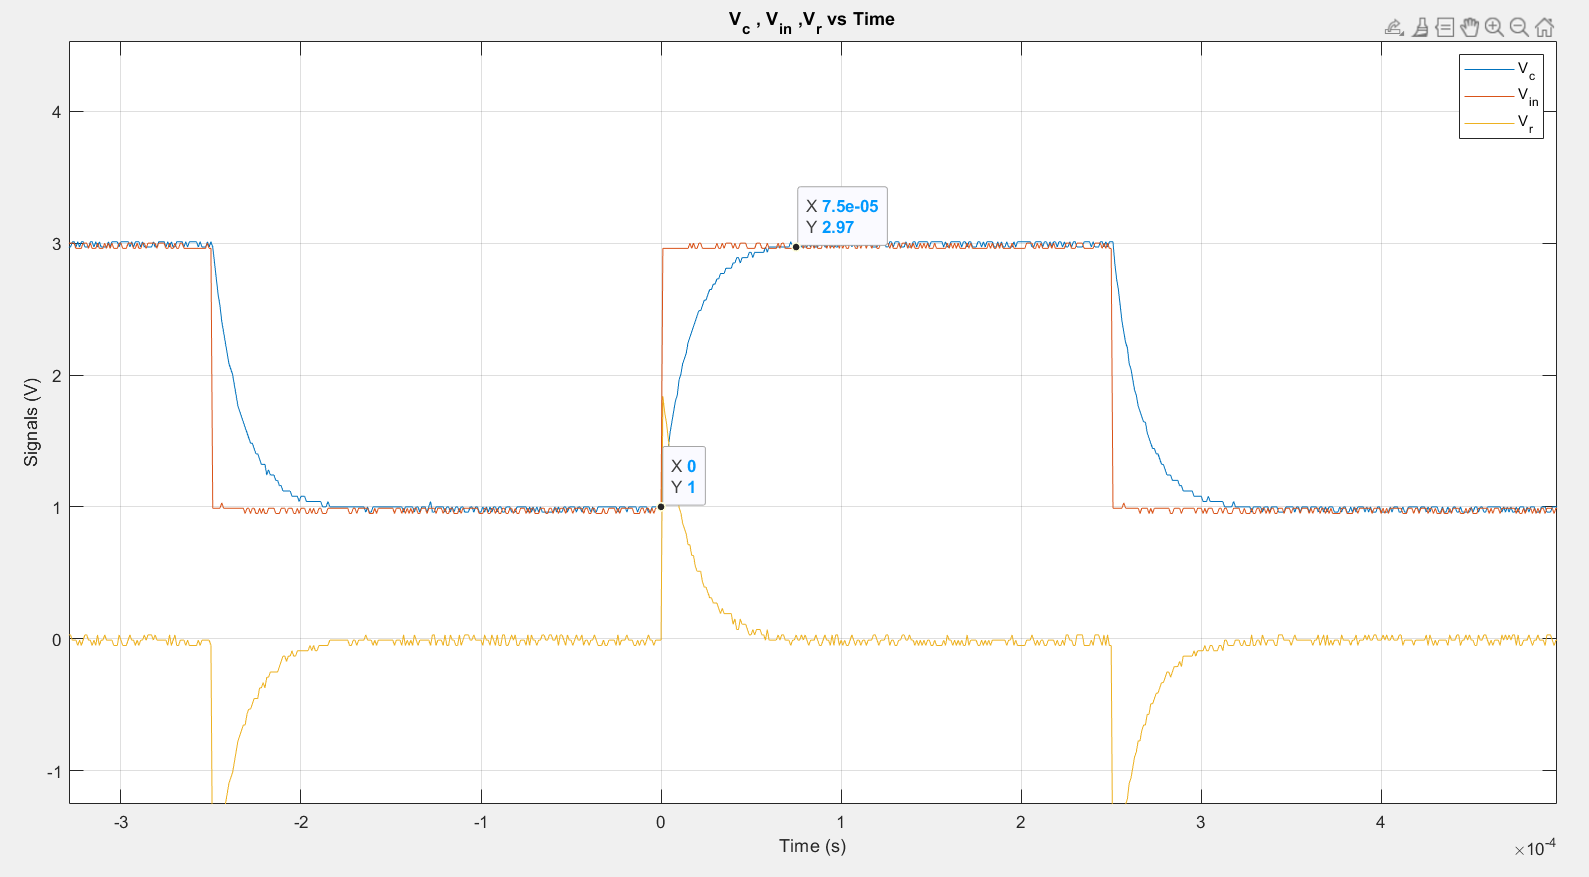
\includegraphics[width=0.8\textwidth]{1_plot_data.png}
   \caption{Data from plot}
\end{figure} 
The result is obtained using 5 \(\tau\) method. The time point where the charging of the capacitor completed is marked. Then it is divided into 5. The calculation result of \(\tau\) is given in Table 2.
\begin{table}[H]
	\begin{center}
	\caption{RC circuit parameters}
	\vspace{2mm}
		\begin{tabular}{||c | c | c | c||} 
		 \hline
		 Experimental Calculation \(\tau\) (\(\mu\) sec & Theoretical Calculation \(\tau\) (\(\mu\) sec) \\ [0.5ex] 
		 \hline\hline
		 15 & 15.51 \\ 
		 \hline
	\end{tabular}
	\end{center}
	\end{table}
It can be stated that 5 \(Tau\) method is consistent with the theoretical calculations. \\

The result of the circuit with parameters of third row is given in Figure 5.

\begin{figure}[H]
	\centering
   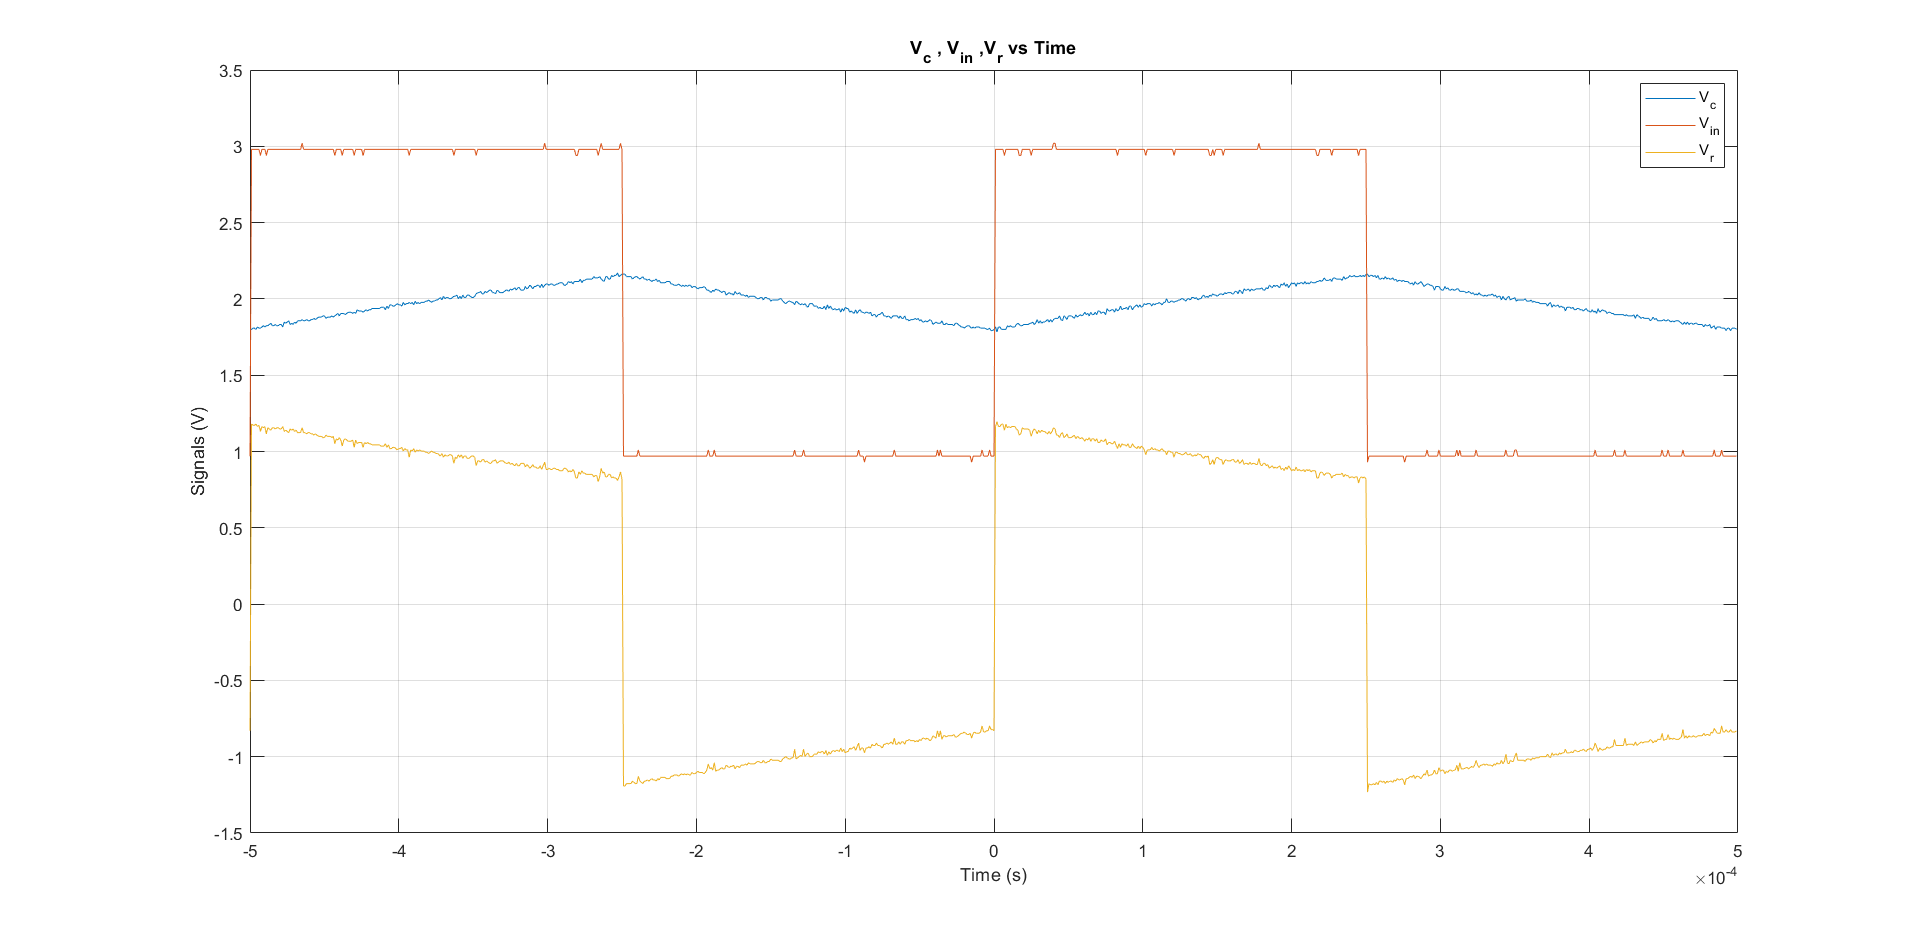
\includegraphics[width=0.8\textwidth]{1a_3.png}
   \caption{Second waveform for the step 1}
\end{figure} 
To measure time constant experimentally following data is obtained from the plot.
\begin{figure}[H]
	\centering
   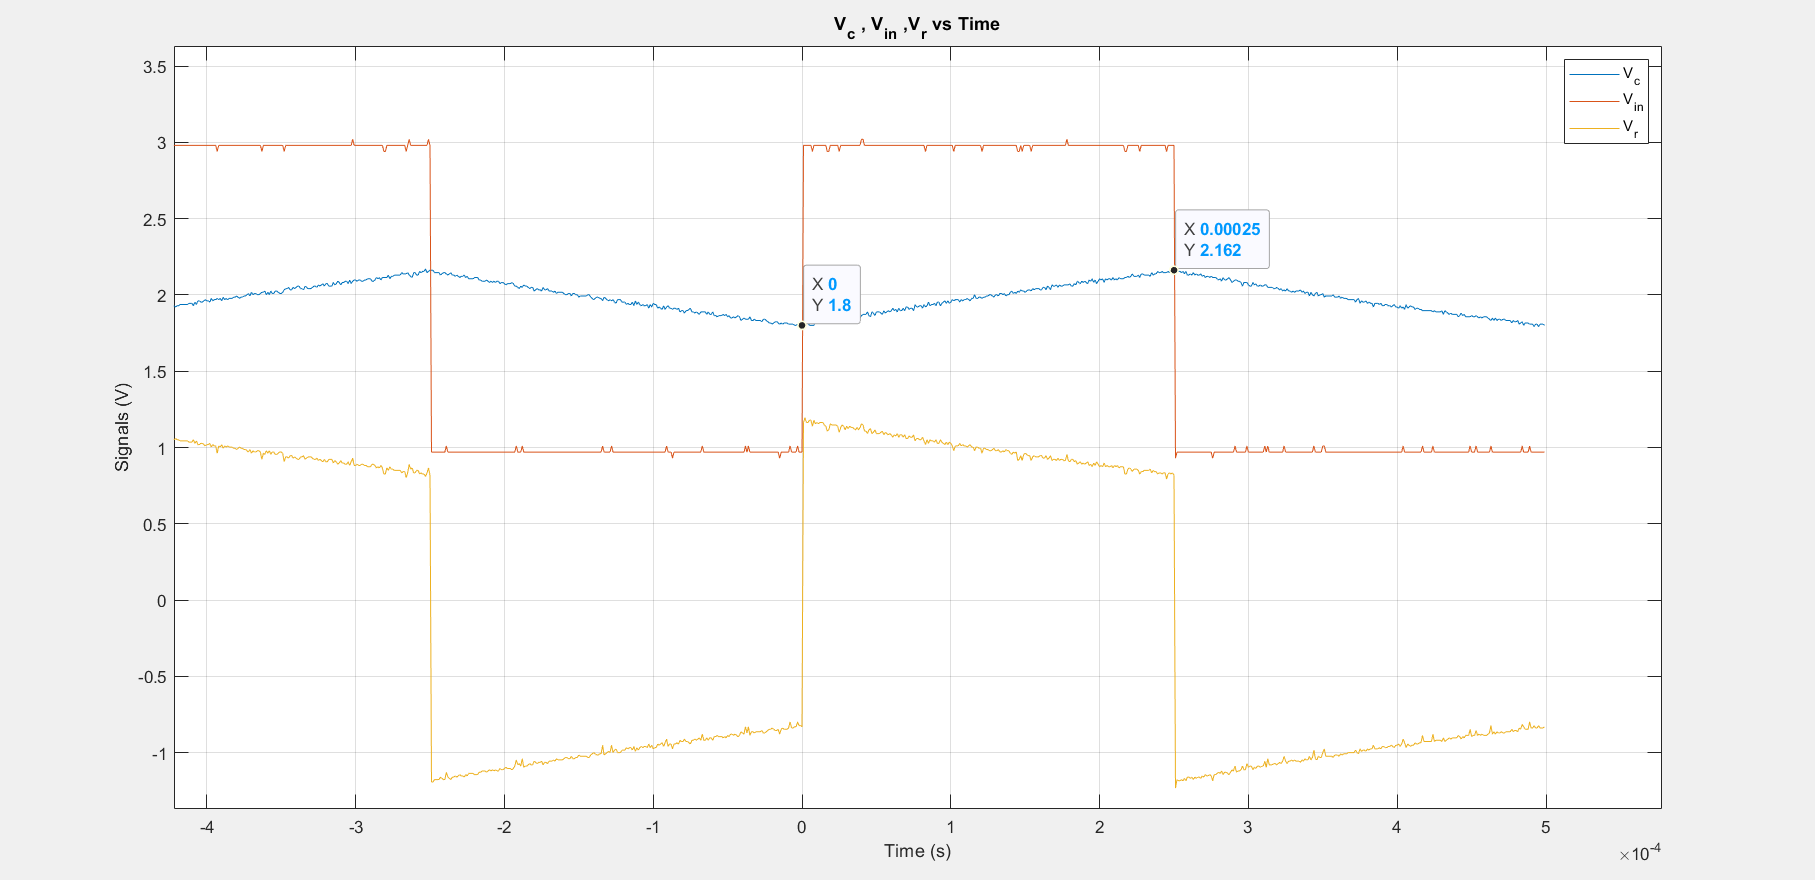
\includegraphics[width=0.8\textwidth]{1_3_plot_data.png}
   \caption{Data from plot}
\end{figure} 
The calculation result of \(\tau\) is given in Table 3. The \(\tau\) can not be obtained using 5 \(\tau\) method because of the fact that charging and discharging proccesses are not completed in a cycle. To obtain the \(\tau\) value both graph data and the equation \(V_c(t)= 3- 2.2 e^-\frac{t}{\tau}\) are used. The time points where the charging and the discharging of the capacitor are marked. When a half cycle is completed 0.25 millisecond passes, so when we set t to 0.25 millisecond we should get the \(V_c\) = 2.162 Volts. The calculation result of \(\tau\) is given in Table 3.
\begin{table}[H]
	\begin{center}
	\caption{RC circuit parameters}
	\vspace{2mm}
		\begin{tabular}{||c | c | c | c||} 
		 \hline
		 Experimental Calculation \(\tau\) (\(\mu\) sec & Theoretical Calculation \(\tau\) (\(\mu\) sec) \\ [0.5ex] 
		 \hline\hline
		 969 & 680 \\ 
		 \hline
	\end{tabular}
	\end{center}
	\end{table}
It can be concluded that our theoretical calculations are quite consistent with the experimental results.

\subsubsection{b)}
For this part, the capacitor  element in the previous part is replaced with an inductor. Apart from capacitor-inductor swap general outline of the setup is conserved.
The set of data given in Table 4 is used for the measurements.

\begin{table}[H]
\begin{center}
\caption{RC circuit parameters}
\vspace{2mm}
	\begin{tabular}{||c | c | c | c||} 
	 \hline
	 \emph{f} (kHz) & R (k\(\Omega\)) & L (H) & Theoretical Calculation \(\tau\) \(\mu\) sec) \\ [0.5ex] 
	 \hline\hline
	 2 & 3.3 & 0.1 & 0.3 \\ 
	 \hline
	 10& 3.3 & 0.1  &   0.3 \\
	 \hline
\end{tabular}
\end{center}
\end{table}
The theoretical calculation of H are obtained from the general time constant equation of RL circuits;
\[\tau = \frac{L}{R}\]
The result of the circuit with parameters of first row is given in Figure 7.

\begin{figure}[H]
	\centering
   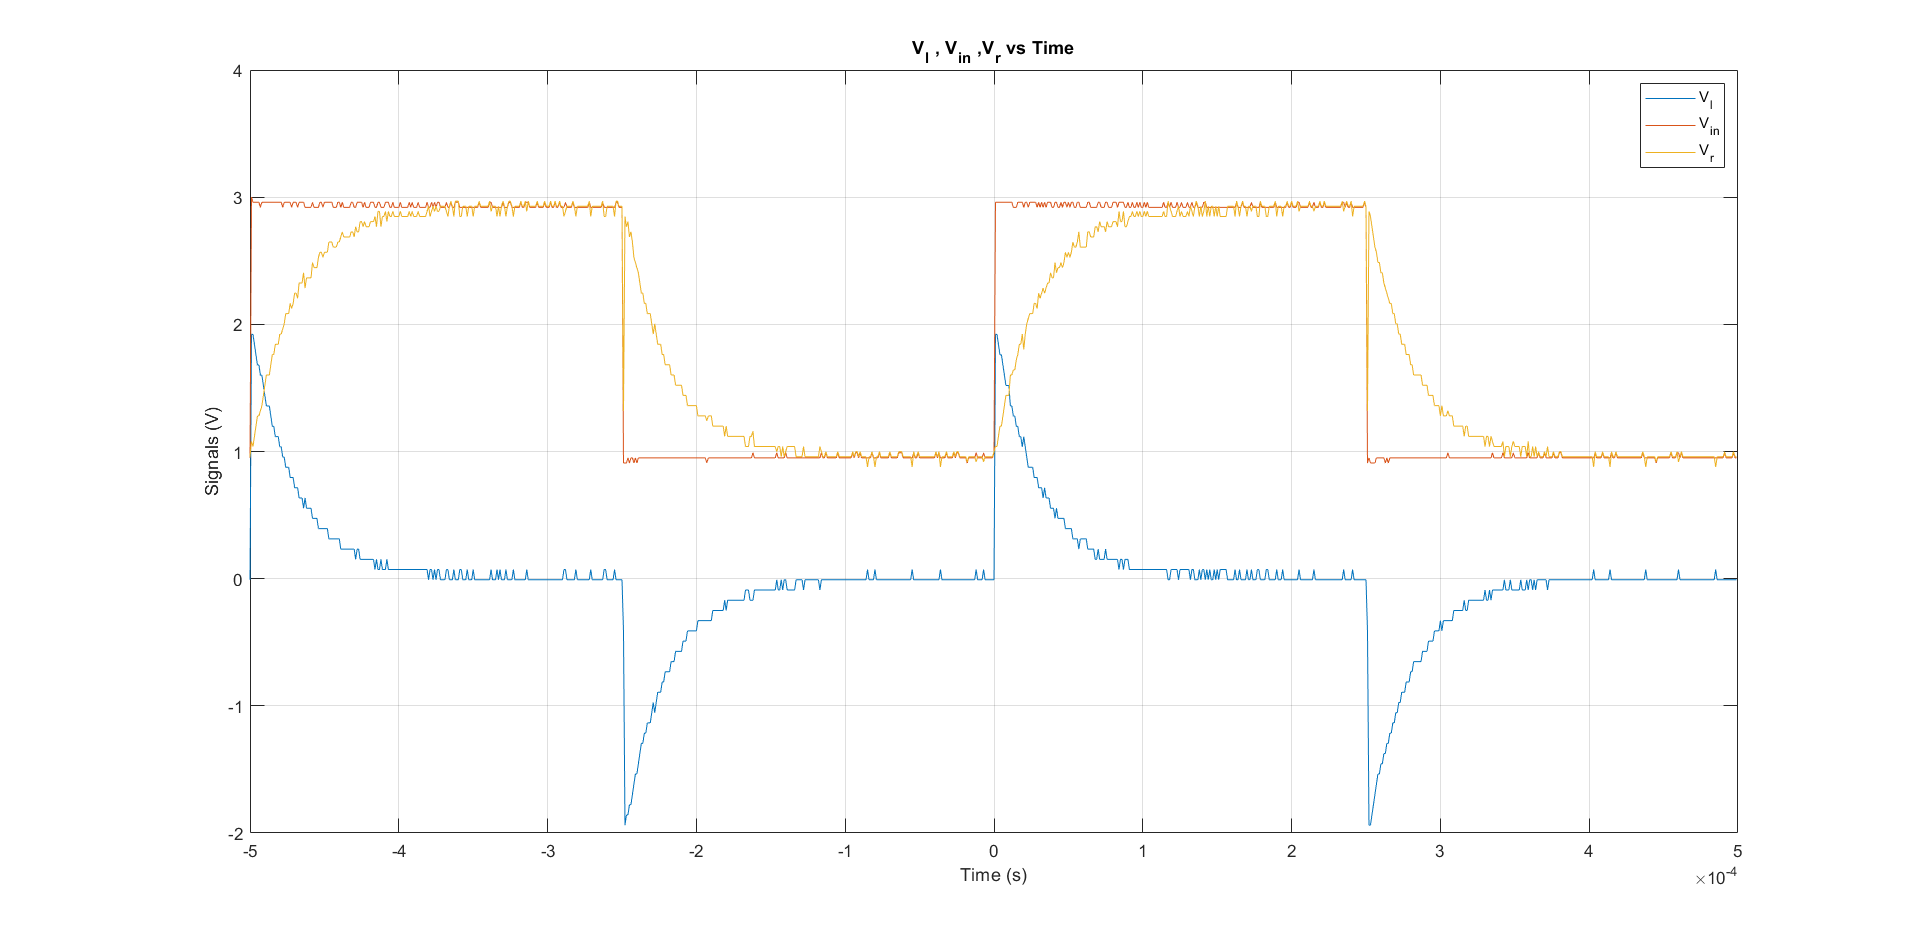
\includegraphics[width=0.8\textwidth]{1b.png}
   \caption{Waveform for the step 1 part 1 first row}
\end{figure} 
To measure time constant experimentally following data is obtained from the plot.
\begin{figure}[H]
	\centering
   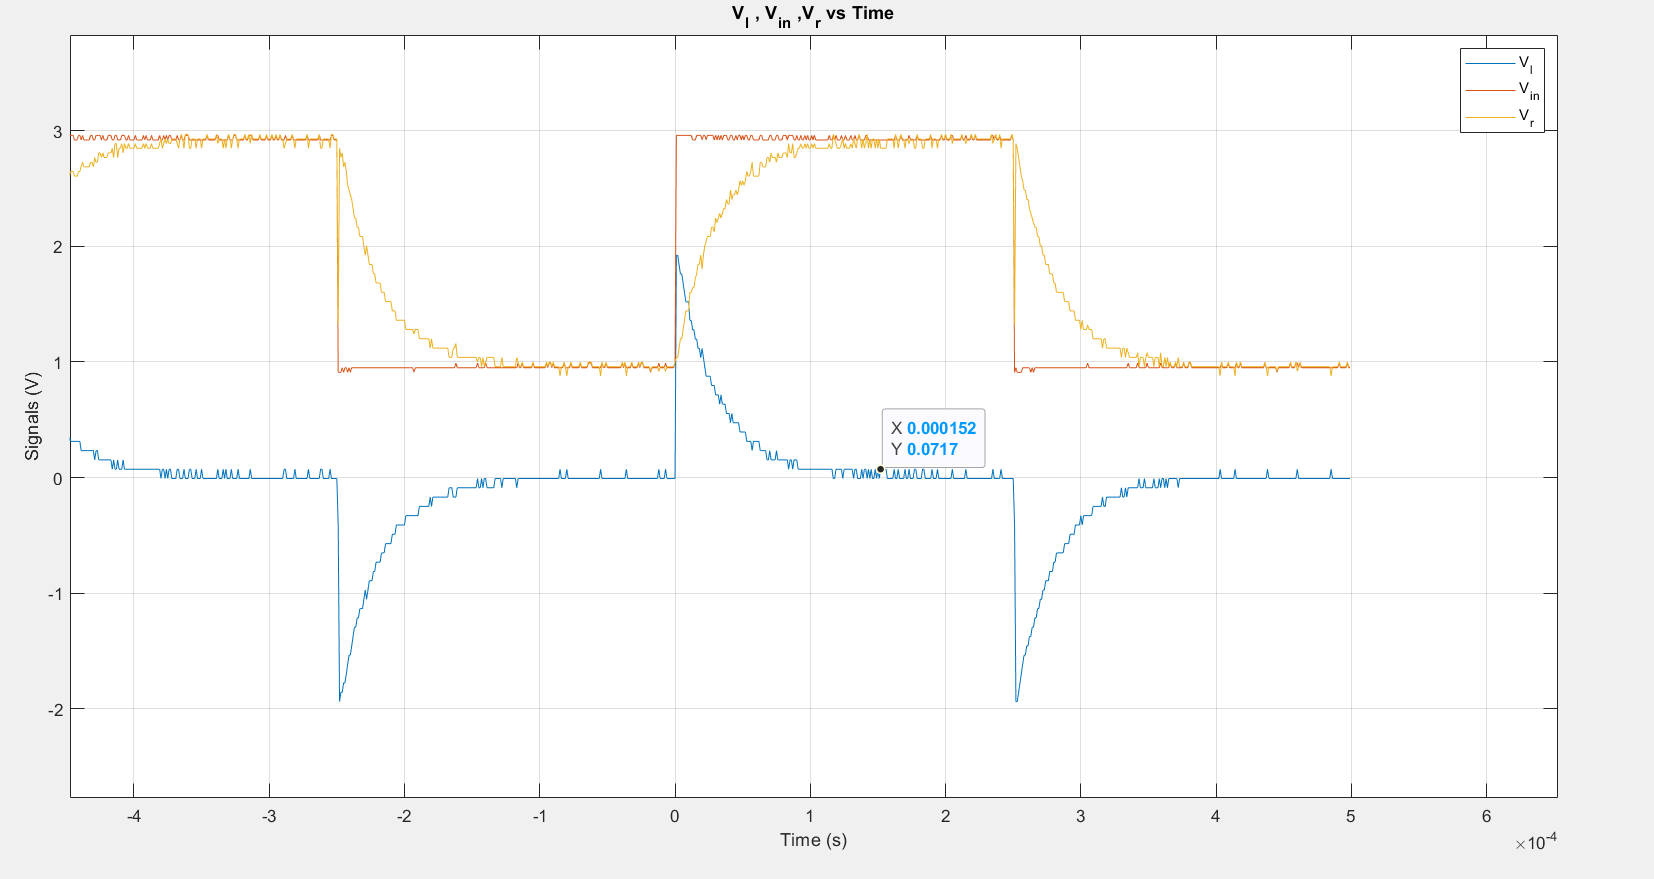
\includegraphics[width=0.8\textwidth]{1_b_plot_data.png}
   \caption{Data from plot}
\end{figure} 

The result is obtained using 5 \(\tau\) method. The time point where the charging of the capacitor completed is marked. Then it is divided into 5. The calculation result of \(\tau\) is given in Table 5.
\begin{table}[H]
	\begin{center}
	\caption{RC circuit parameters}
	\vspace{2mm}
		\begin{tabular}{||c | c | c | c||} 
		 \hline
		 Experimental Calculation \(\tau\) (\(\mu\) sec & Theoretical Calculation \(\tau\) (\(\mu\) sec) \\ [0.5ex] 
		 \hline\hline
		 0.303 & 0.3 \\ 
		 \hline
	\end{tabular}
	\end{center}
	\end{table}
It can be said that 5 \(Tau\) method is consistent with the theoretical calculations. \\
The result of the circuit with parameters of third row is given in Figure 5.

\begin{figure}[H]
	\centering
   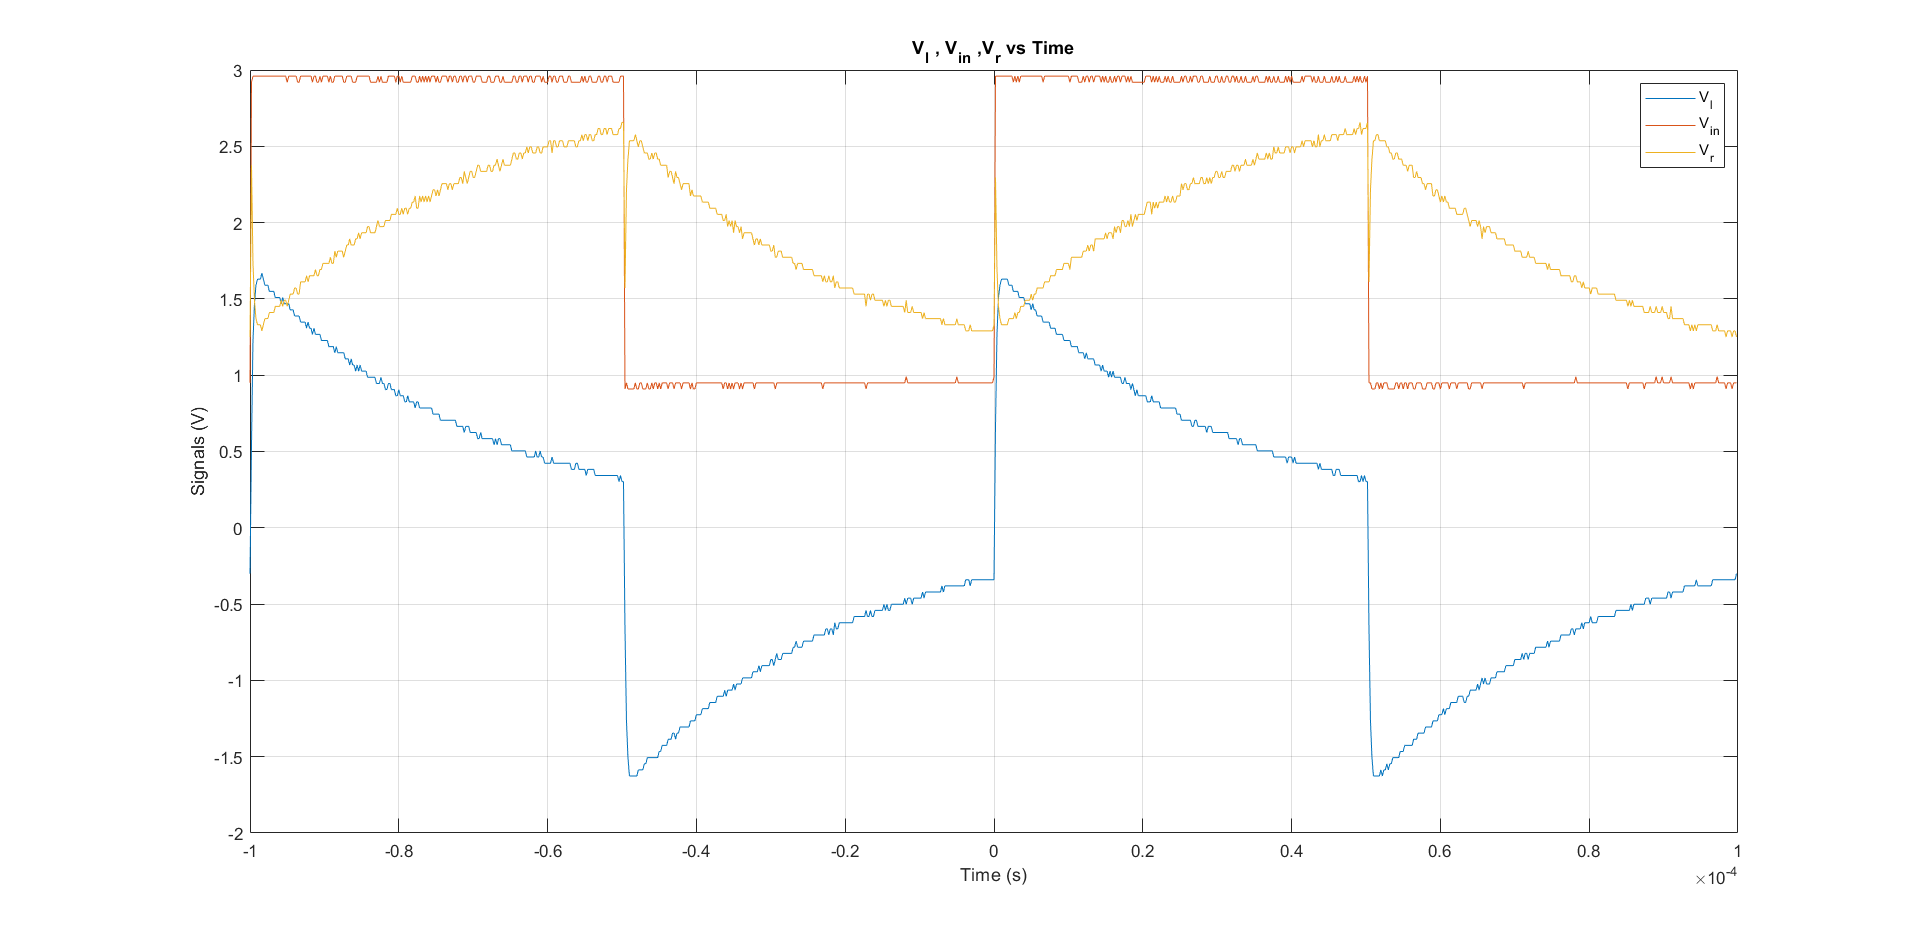
\includegraphics[width=0.8\textwidth]{1b_3.png}
   \caption{Second waveform for the step 1 part b}
\end{figure} 
To measure time constant experimentally data in Figure 9 is obtained from the plot.
\begin{figure}[H]
	\centering
   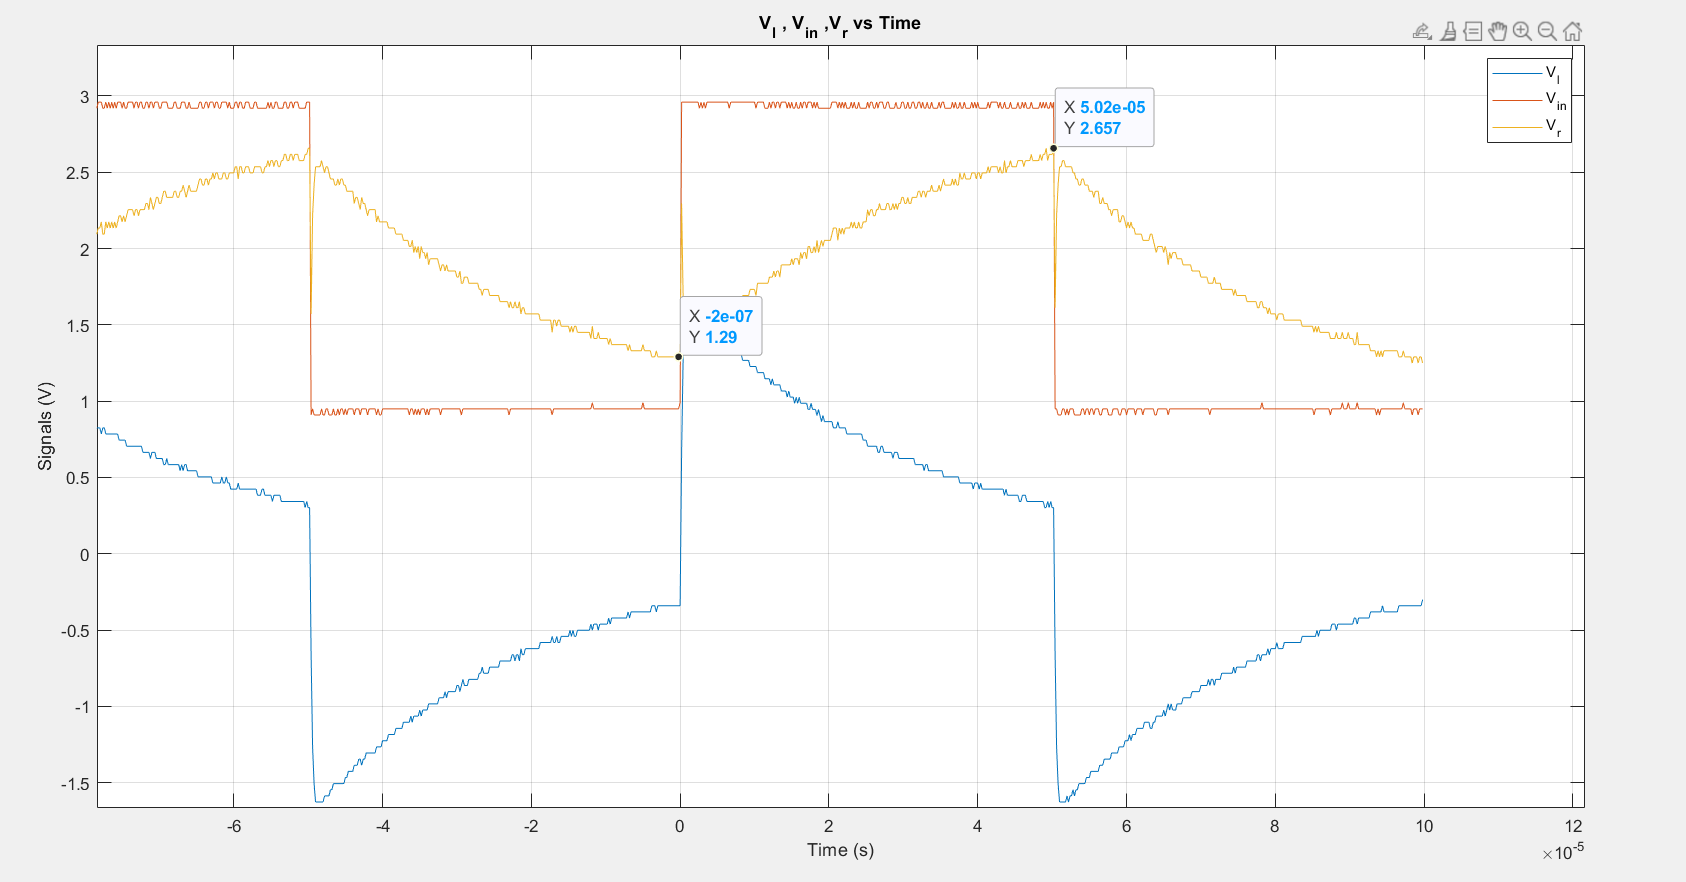
\includegraphics[width=0.8\textwidth]{1_b_3_plot_data.png}
   \caption{Data from plot}
\end{figure} 
The calculation result of \(\tau\) is given in Table 6. The \(\tau\) can not be obtained using 5 \(\tau\) method because of the fact that charging and discharging proccesses are not completed in a cycle. To obtain the \(\tau\) value both graph data and the equation \( i_c (t) = 10^{-3} * (1 - 0.609 e^-\frac{t}{\tau}) \)  are used. The time point where the charging and the discharging of the inductor is marked. When a half cycle is completed 0.05 millisecond passes, so when we set t to 0.05 millisecond we should get the \( i_c  = 0.8052*10^-3\) Amps. The calculation result of \( \tau \) is given in Table 6 .
%
\begin{table}[H]
	\begin{center}
	\caption{RC circuit parameters}
	\vspace{2mm}
		\begin{tabular}{||c | c | c | c||} 
		 \hline
		 Experimental Calculation \(\tau\) (\(\mu\) sec )& Theoretical Calculation \(\tau\) (\(\mu\) sec) \\ [0.5ex] 
		 \hline\hline
		 0.437 & 0.303 \\ 
		 \hline
	\end{tabular}
	\end{center}
	\end{table}
It can be concluded that our theoretical calculations are quite consistent with the experimental results regarding the error is approximately a tenths of a millisecond.

\subsection{2}
The circuit given in Figure 11 is constructed. Function generator is adjusted so that it supplies square waves with frequency of 100Hz and \(V_{pp}\) = 6Volts. 
\begin{figure}[H]
	\centering
   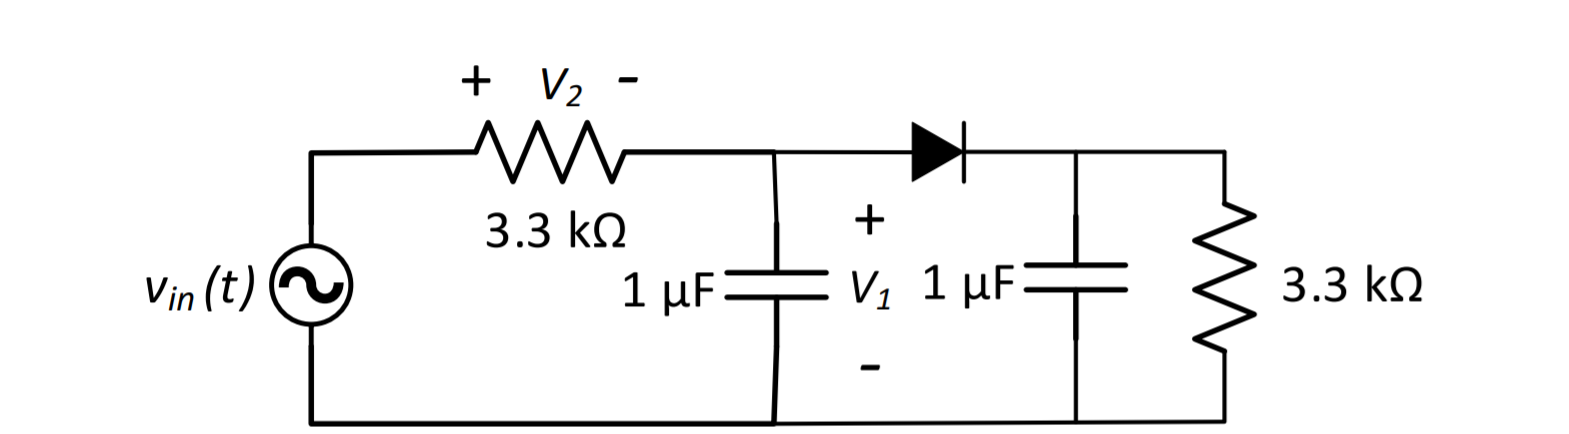
\includegraphics[width=0.8\textwidth]{2_sch.png}
   \caption{Circuit schematic for step 2}
\end{figure} 
Then the plot shown in Figure 12 is obtained.
\begin{figure}[H]
	\centering
   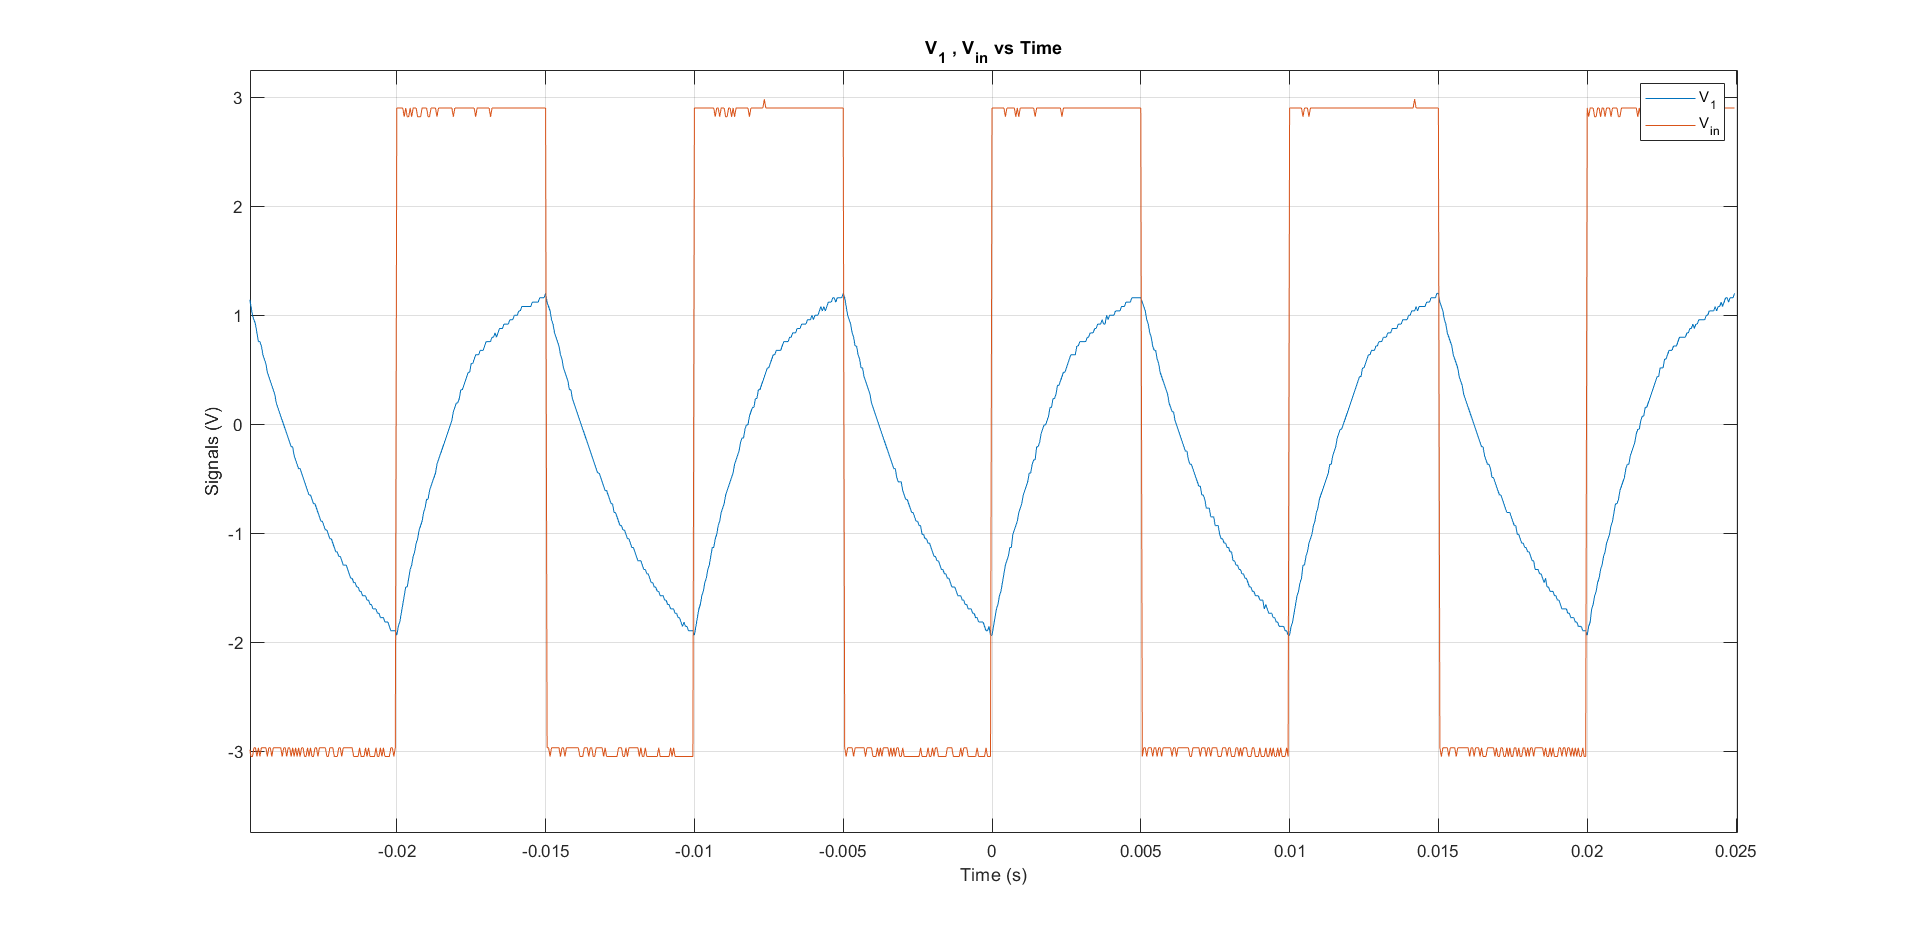
\includegraphics[width=0.8\textwidth]{2.png}
   \caption{\(V_1\) and \(V_{in}\) vs Time}
\end{figure} 
Now, the time constant \(\tau\) can be obtained for two states of which signal is positive and negative. For negative region it can be calculated theoretically easily by multiplying R and C. On the other hand for positive region it can be obtained after finding thevenin equivalent of the circuit. But, those values also can be obtained from the plot given in Figure 12. To do this the measurements on the plot is made and given in Figure 13.
\begin{figure}[H]
	\centering
   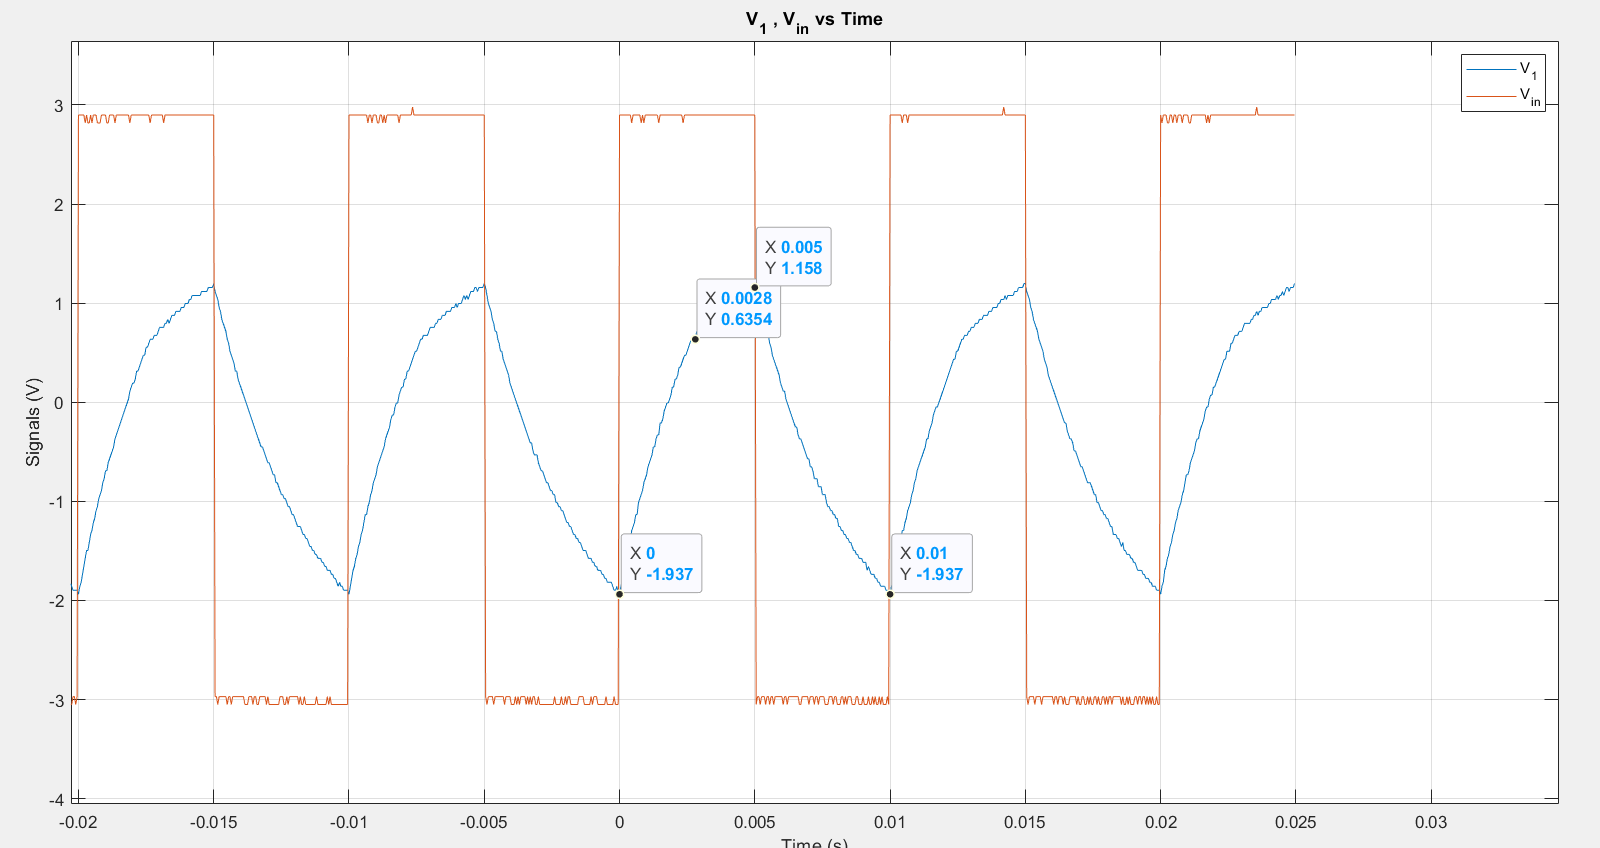
\includegraphics[width=0.8\textwidth]{2_plot_data.png}
   \caption{Data marks for the step 2}
\end{figure} 
Again, for this step 5 \(\tau\) method can not be used since the period of charge and discarge is not complete.
For positive region the equation is;
\[V_c = 3 - 4.937e^-\frac{t}{\tau_+}\]
\[1.158 = 3 - 4.937e^{-\frac{0.005}{\tau_+}} \]
For negative region the equation is, 
\[V_c = -3 + 4.158e^-\frac{t}{\tau_-}\]
\[ -1.937 = - 3 + 4.158e^{-\frac{0.005}{\tau_-}} \]
So the results of experimental calculations are given in Table 7.
\begin{table}[H]
	\begin{center}
	\caption{RC circuit parameters}
	\vspace{2mm}
		\begin{tabular}{|| c | c |c ||} 
		 \hline
		  &Experimental Calculation \(\tau\) ( sec )& Theoretical Calculation \\ [0.5ex] 
		 \hline\hline
		 \(\tau_+\)&\(5.07*10^{-3}\)&\(3.3*10^{-3}\)    \\ 
	 \hline
	 \(\tau_-\)& \(3.666*10^{-3}\)& \(3.3*10^{-3}\) \\
	 \hline
\end{tabular}
\end{center}
\end{table}
As mentioned, the theoretical results are obtained using several calculations ,but it can be convinient to use experimental approach because of its simplicity. To sum up, the circuit operates in positive and negative regions. In positive region, both of the capacitors are charging. In negative region both of the capacitors are discharging but while left capacitor charges from opposite direction, right capacitor discharge its energy to rightmost resistor.  Also the  even though \(\tau\) values of positive region and negetive region are same in theoretical manner, the since the internal resistances and initial conditions of capacitors neglected, there are deviation on the results.

 

\subsection{3}
The circuit given in Figure 14 is taken as the reference for the differentiator setup.
\begin{figure}[H]
	\centering
   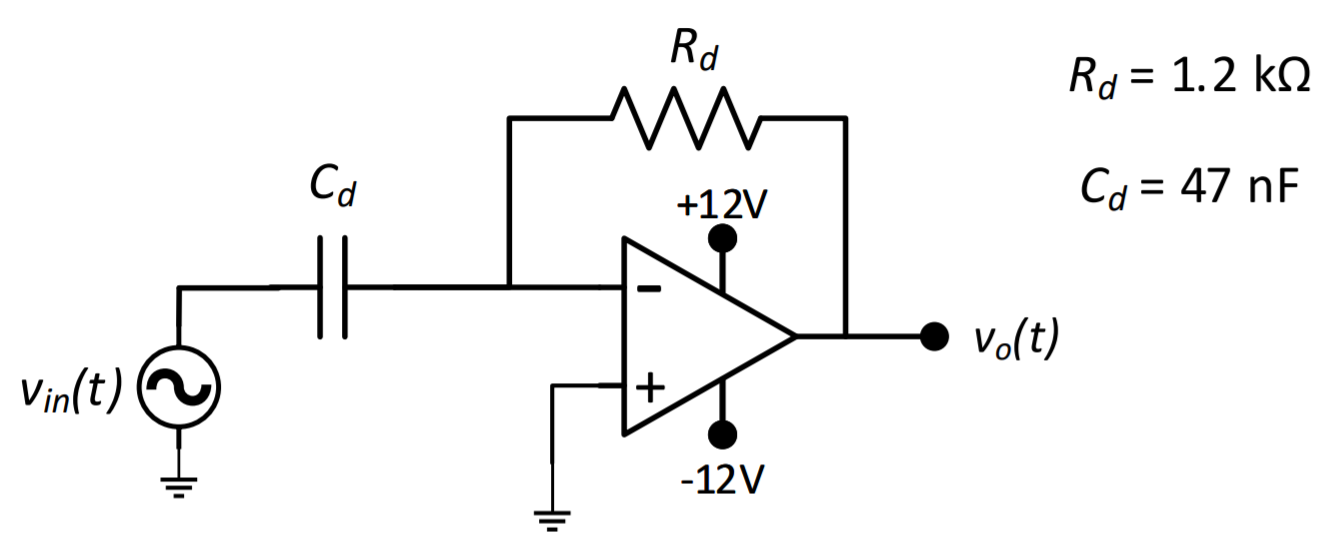
\includegraphics[width=0.8\textwidth]{differentiator.png}
   \caption{Differentiator circuit schematic}
\end{figure} 
Then the circuit is constructed in LTSpice environment which is shown in Figure 15.
\begin{figure}[H]
	\centering
   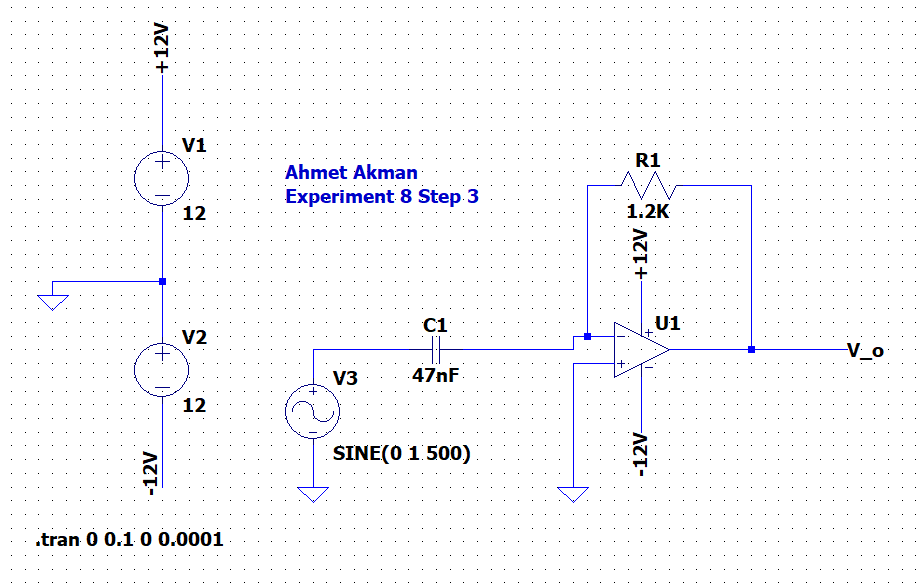
\includegraphics[width=0.8\textwidth]{differentiator_sim.png}
   \caption{Differentiator circuit in LTSpice}
\end{figure} 
Then the input versus output characteristics are obtained as given in Figure 16.
\begin{figure}[H]
	\centering
   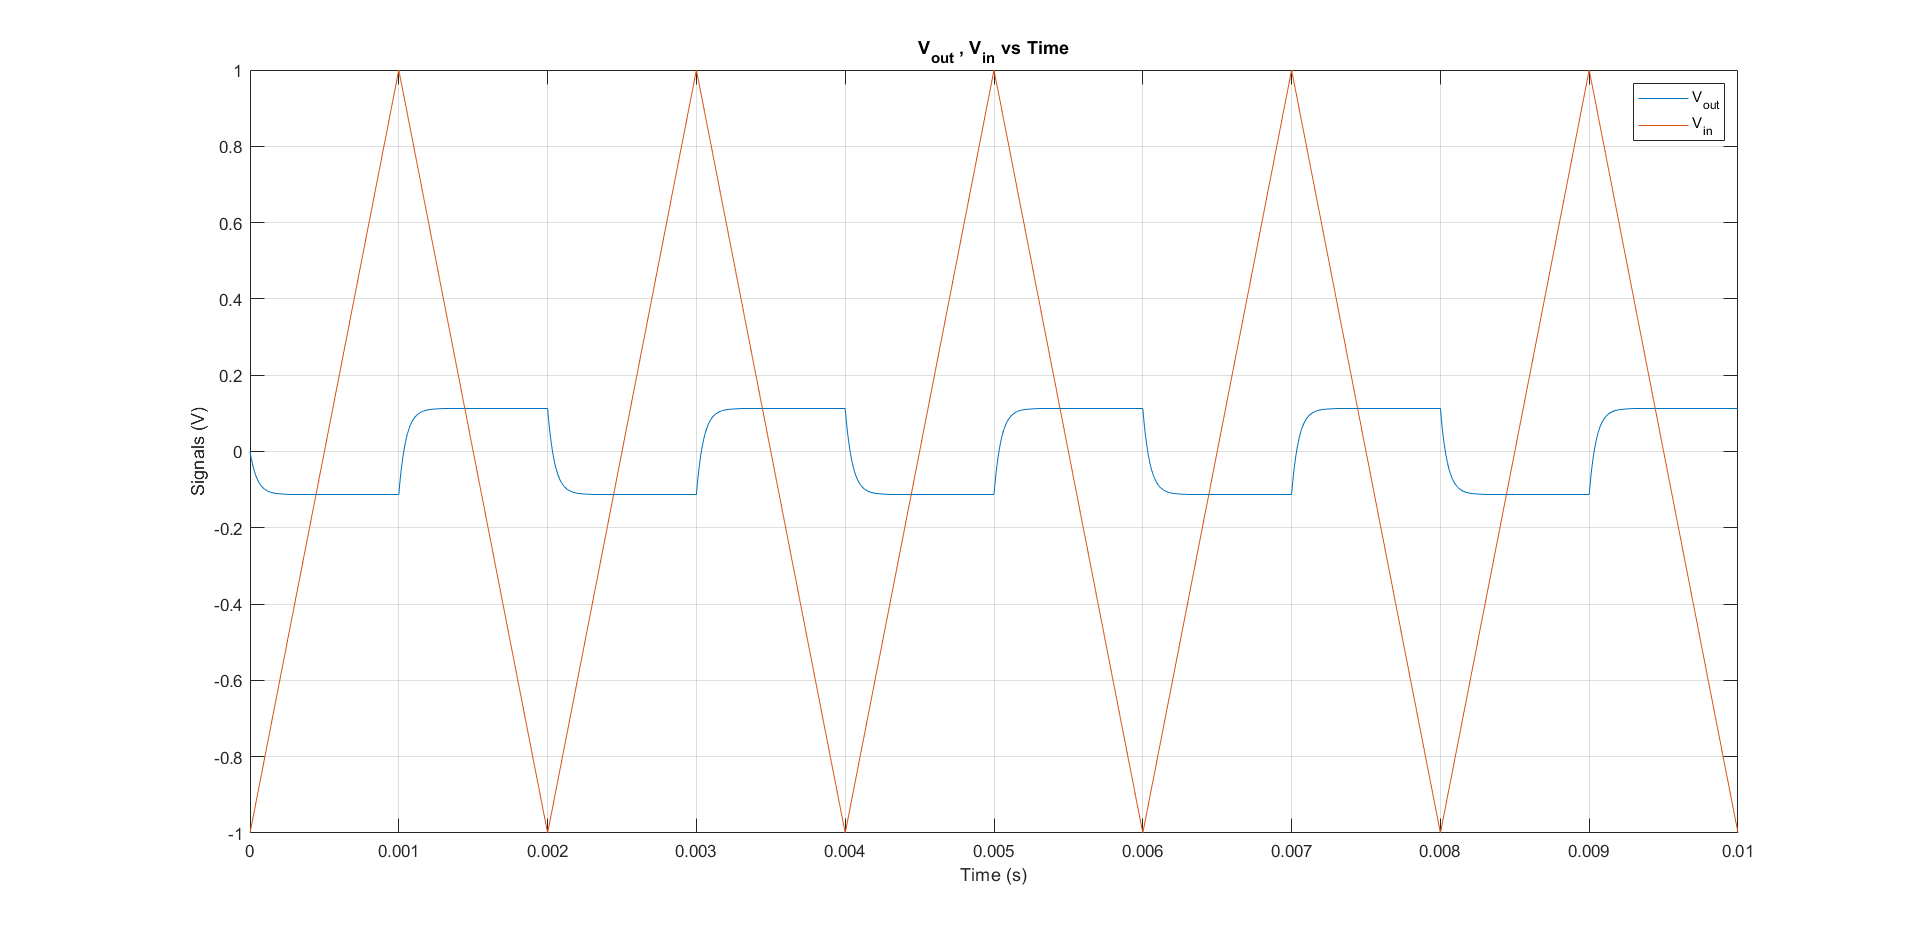
\includegraphics[width=0.8\textwidth]{differentiator_1.png}
   \caption{Differentiator circuit output}
\end{figure} 
As a result, it can be said that this circuit configuration is able to differentiate the given signal. Because of the non-ideality of the components (e.g. internal resistance of the capacitor) the resulting signal is not exactly square wave.  The differentiation of a triangular wave is a square wave as observed. So, the expression relating signal is as follows,
\[V_{out} = \frac{dV_{in}}{dt}\]
\newline
The circuit shown in Figure 17 is constructed.
\begin{figure}[H]
	\centering
   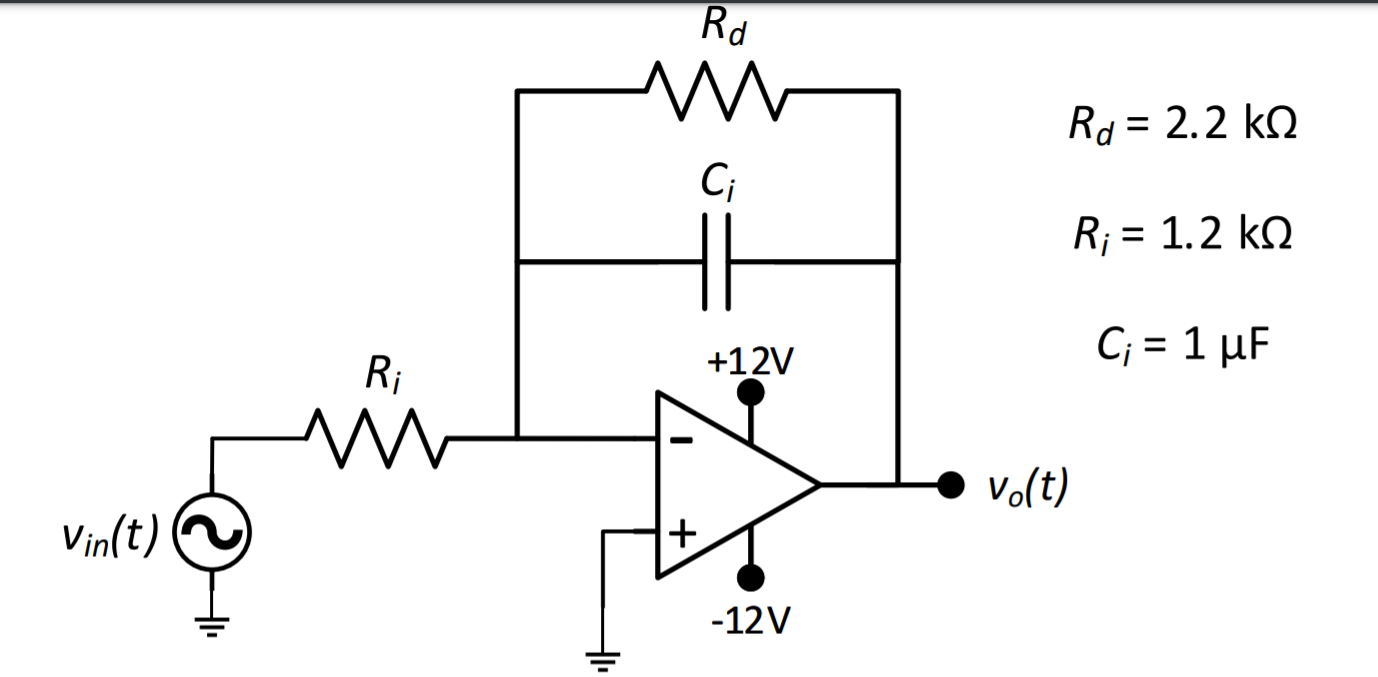
\includegraphics[width=0.8\textwidth]{integrator.png}
   \caption{Integrator circuit schematic}
\end{figure} 
Then the output plot given in Figure 18 is obtained.
\begin{figure}[H]
	\centering
   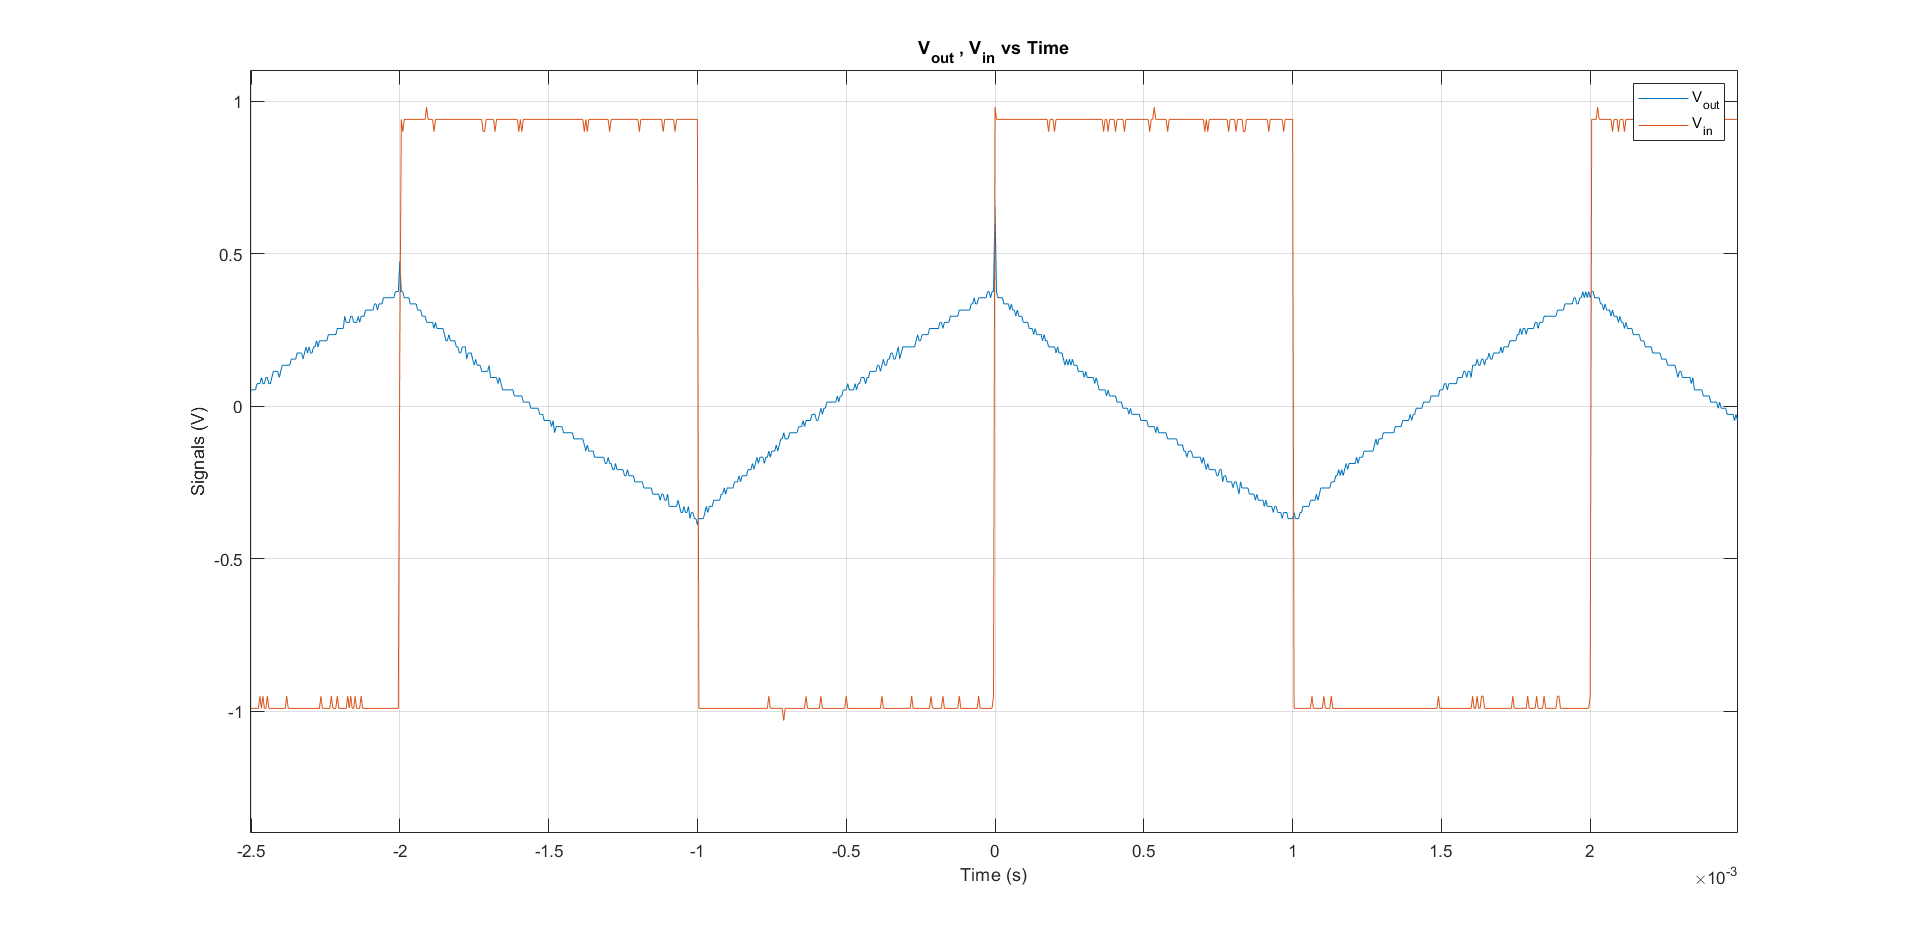
\includegraphics[width=0.8\textwidth]{3.png}
   \caption{Integrator circuit output}
\end{figure} 
As a result it can be said that this circuit setup integrates the input signal ,so that output signal is oscillating between 0.3 V and 0.3 V approximately. The integration of the square wave is the triangular wave as observed.
\section{Conclusion}

In conclusion, in experiment 8, "First Order Circuits," as students, we have learned how various RC and RL circuit setup constructed. As students, we have seen how the time constant \(\tau\) can be determined from the plot. We have inferred the time constance of RC and RL circuits experimentally and compared them with the theoretical ones. The 5 \(\tau\) method is used and observed when it can not be used. Then, the behavior of a RC circuit with a diode observed and commented on.  Lastly, basic differential circuits and their behaviors are observed, and the mathematical expressions are verified by signal outputs. To sum up, in this experiment, as students, we have experimented with various RC circuits and their responses, then we have compared them with the expected responses. 
\section*{Appendix I}
Total time spent on/during:
\begin{itemize} 

	\item Report writing: 10 hours 
\end{itemize}
\section*{Appendix II}
The outputs of the simulations are fetched from LTSpice and plotted in MATLAB. 
%++++++++++++++++++++++++++++++++++++++++
% References section will be created automatically 
% with inclusion of "thebibliography" environment
% as it shown below. See text starting with line
% \begin{thebibliography}{99}
% Note: with this approach it is YOUR responsibility to put them in order
% of appearance.

%\begin{thebibliography}{99}

%https://tr.overleaf.com/latex/templates/sample-lab-report-for-u-of-r-phys-349/pgsyqngcyjxk

%\end{thebibliography}


\end{document}


\begin{table}[H]
	\begin{center}
		\caption{Resistance reading by color code convention.}
		\vspace{2mm}
		\begin{tabular}{||c | c | c||} 
		 \hline
		 Color Order & Value & Tolerance \\ [0.5ex] 
		 \hline\hline
		 Brown / Black / Red / Gold & 1k\( \Omega \) & \( \% \) 5  \\ 
		 \hline
		 Yellow / Violet / Red / Gold & 4.7k\( \Omega \) & \( \% \) 5   \\
		 \hline
		 Brown / Grey / Orange / Gold & 18k\( \Omega \) & \( \% \) 5  \\ [1ex] 
		 \hline
		\end{tabular}
	\end{center}
	\end{table}
	

	\begin{figure}[H]
 		\centering
		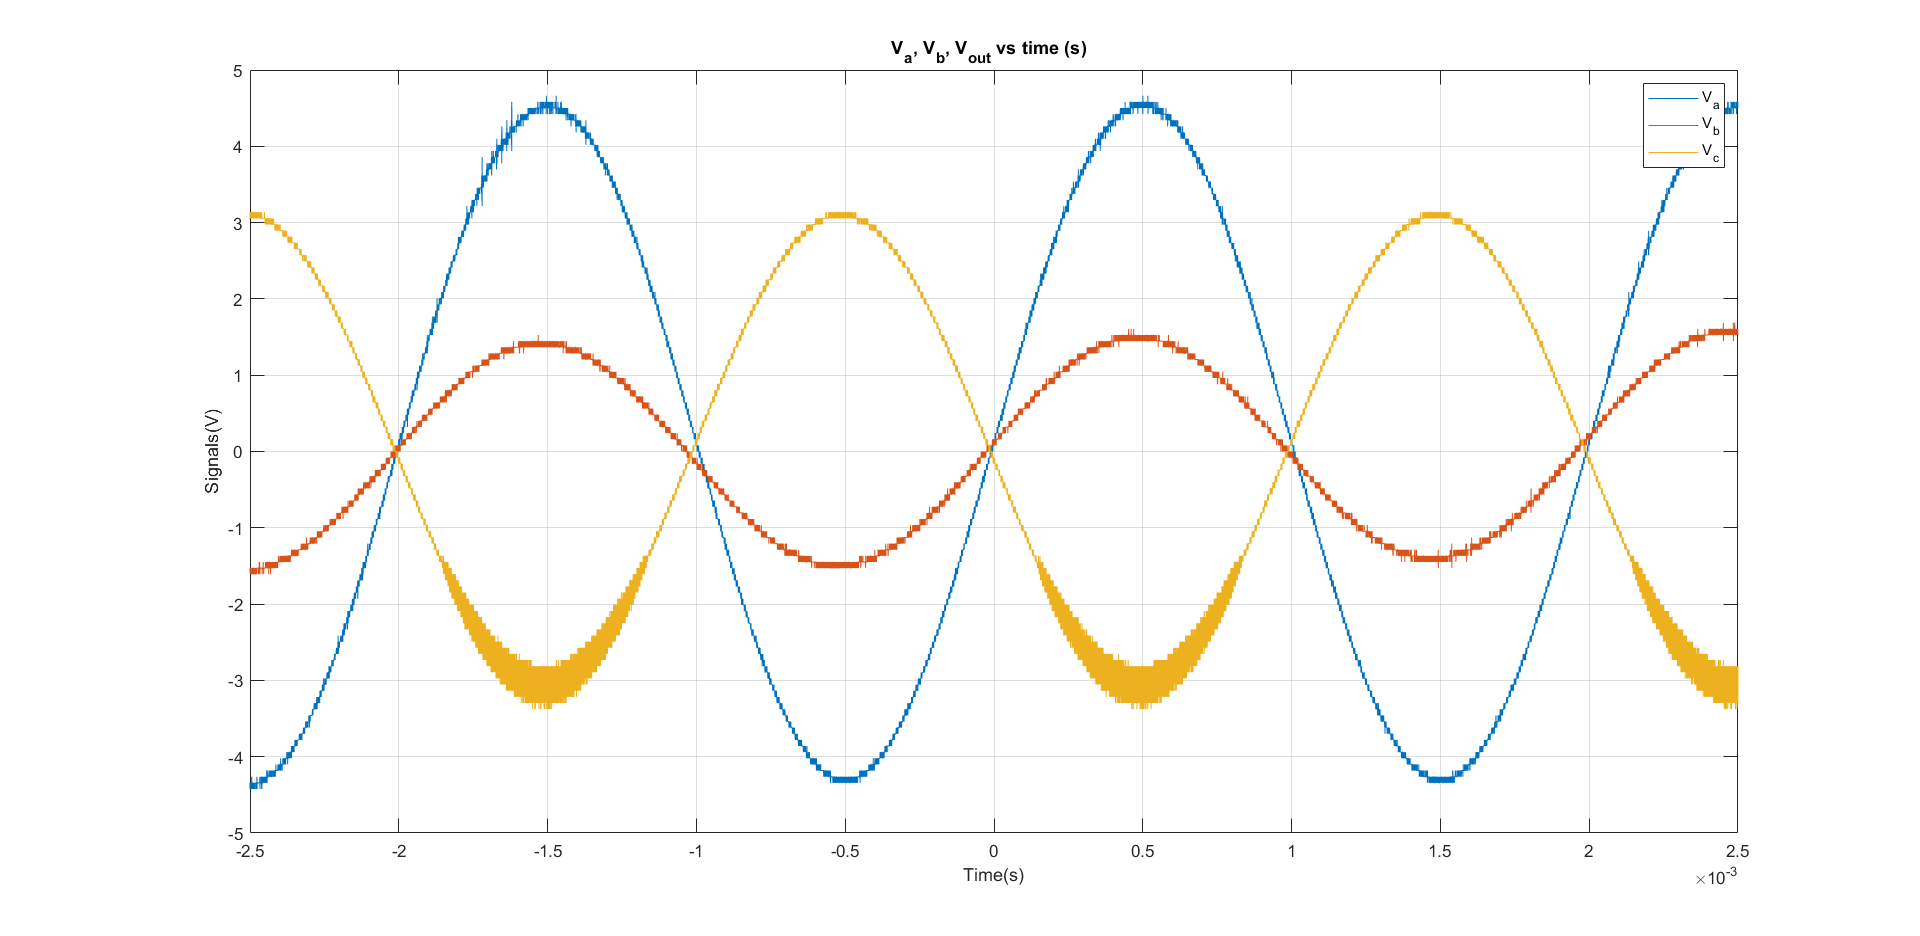
\includegraphics[width=0.6\textwidth]{5.png}
		\caption{Circuit schematic for the step 5}
	\end{figure} 

	\begin{figure}[htp] \centering{
		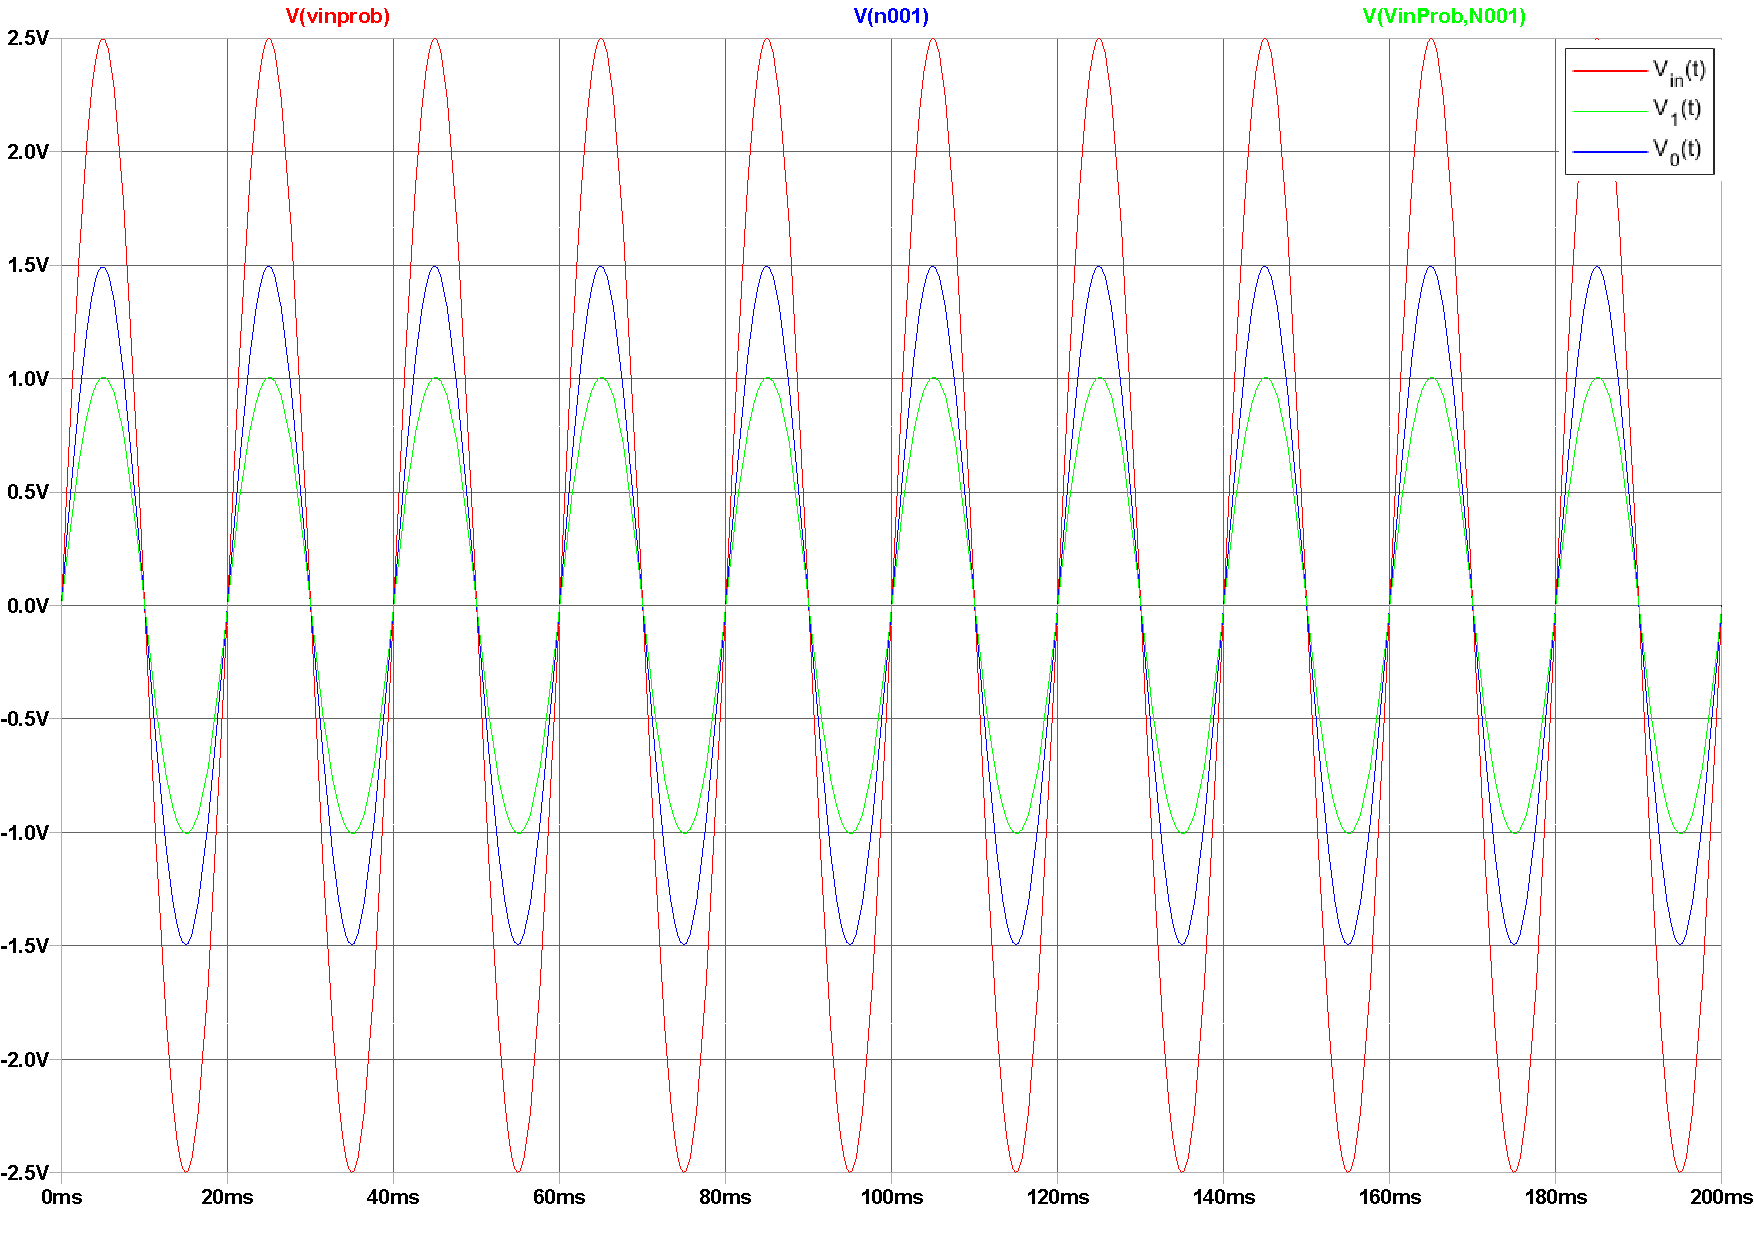
\includegraphics[scale=0.25]{2a_plot.pdf}}
		\caption{Experiment 2}
\end{figure}
	